\documentclass[11pt]{article}
\usepackage[a4paper,margin=1in]{geometry}
\usepackage{amsmath,amssymb,amsthm,mathtools}
\usepackage{booktabs}
\usepackage{enumitem}
\usepackage{float}
\usepackage{graphicx}
\usepackage{hyperref}
\usepackage[nameinlink,capitalise]{cleveref}
\usepackage[numbers,sort&compress]{natbib}

\newtheorem{theorem}{Theorem}[section]
\newtheorem{proposition}[theorem]{Proposition}
\newtheorem{corollary}[theorem]{Corollary}
\newtheorem{condition}[theorem]{Condition}
\theoremstyle{remark}
\newtheorem{remark}[theorem]{Remark}

\newcommand{\norm}[1]{\left\lVert#1\right\rVert}
\newcommand{\HS}{\mathfrak S_2}
\newcommand{\cE}{\mathcal E}
\newcommand{\tr}{\operatorname{tr}}
\newcommand{\spr}{\operatorname{spr}}

\title{Time-Ordered Schur Cross-Gramians for Directional Hardy Fusion\\
\large Removing Radial Riesz Obliqueness}
\author{Liang Wang}
\date{July 2026}

\begin{document}
\maketitle

\begin{abstract}
RH-57 expressed directional Hardy energies through cross-Gramians built from
invariant Riesz blocks.  Its fixed radial projectors became severely oblique
as the noise decreased.  This paper replaces those projectors by a unitary
ordered Schur basis and identifies exactly what that replacement gains and
what it does not.

For each stable finite matrix $A=QTQ^*$, we prove two dual positive packet
identities for every orthogonal coordinate partition of its triangular Schur
form.  The input identity decomposes the complete response into
orthogonal initial Schur packets through the observability Gramian; the output
identity decomposes the controllability Gramian into observed Schur state
blocks.  Both reconstruct the same Hardy energy and admit coherence-weighted
square-sum bounds.  We also prove a reverse-order cross-Stein recursion for
the blocks of the controllability Gramian.  A block-power formula bounds every
diagonal Stein inverse without forming a Kronecker matrix.

The deterministic five-scale binary64 audit is sharply positive at the exact
packet level.  At the smallest stored scale, the left/right input-packet
coherence uppers are $1.5527$ and $1.9009$, while the output-block uppers are
$1.4682$ and $1.7612$.  The corresponding RH-57 radial Riesz uppers were
$81.68$ and $672.41$.  Every diagonal Schur block has eight-step norm below
$0.290$, and the largest observed block-Stein gain is below $2.80$.

There is also a new negative result.  If every feed-forward Schur path is
replaced by spectral/Frobenius norms and summed absolutely, the sufficient
upper grows to $1922.4$ and $380.4$.  Thus unitary Schur coordinates remove
Riesz obliqueness, but a scalar absolute-path proof discards the packet
orthogonality that made the decomposition useful.  A 256-bit Arb calculation
certifies the formulas on a two-scalar-block model only.  No dyadically
uniform physical packet theorem, Stage A1 closure, arithmetic trace formula,
or Hilbert--Polya conclusion is claimed.
\end{abstract}

\noindent\textbf{Keywords:} Schur form; cross-Gramian; Stein equation;
Hardy energy; Haar channel; nonnormal operator; small noise.

\medskip
\noindent\textbf{MSC 2020:} 47A10; 47B65; 37D25; 37M25; 65F35.

\section{Introduction}

The intrinsic small-noise program has reduced its remaining analytic premise
to two directional Hilbert--Schmidt Hardy energies.  RH-48--RH-50 derived the
Schur-complement and time-domain reductions; RH-51--RH-56 supplied finite
Stein tails, residue and cutoff transfer, and a quantitative obstruction to a
global strong-space argument \citep{WangIntrinsic2026,WangDirectional2026,
WangHardy2026,WangStructuredStein2026,WangFactorTransfer2026,
WangHardyTail2026,WangFactorAware2026,WangRieszCutoff2026,
WangHardyBarrier2026}.  RH-57 then proved an exact Riesz cross-Gramian identity
and tested fixed radial invariant blocks \citep{WangRieszOverlap2026}.

The RH-57 result exposed a precise mismatch.  The exact all-column Hardy
energies remained below $1.77$ on the stored dense levels, but fixed radial
Riesz projectors reached norms above $2.5\times10^3$.  Their individual block
responses became large and cancelled only after aggregation.  Consequently,
an absolute invariant-block budget was not a credible uniform proof route.

The Schur form is the natural next coordinate system
\citep{GolubVanLoan2013,HornJohnson2013}.  It replaces oblique
spectral projections by a unitary basis while retaining a time ordering:
outer spectral packets feed inner packets through the strictly upper block
part of $T$.  This paper answers two separate questions.

\begin{enumerate}[leftmargin=2.2em]
 \item Does the unitary packet decomposition itself remain quantitatively
       mild on the growing finite family?
 \item Can that mild decomposition be proved by taking absolute norms along
       every upper-triangular feed-forward path?
\end{enumerate}

The audit answers yes to the first and no to the second.  This distinction is
the main route information supplied by RH-58.

\subsection*{Contributions and boundary}

\begin{enumerate}[leftmargin=2.2em]
 \item We prove dual input-packet and output-state Gram identities in an
       arbitrary unitary Schur partition.  No diagonalizability is required.
 \item We prove the reverse cross-Stein block recursion induced by upper
       triangularity.
 \item We derive a computable block-power upper for each Stein inverse and a
       rigorous scalar absolute-path majorant.
 \item We audit both exact packet Grams and the scalar path majorant on five
       all-column folded-Gaussian levels, with all primal, dual, Schur, and
       recursion residuals stored.
\end{enumerate}

The finite-dimensional identities are exact.  The ordered production Schur
forms are binary64 and noise-dependent.  Nothing below proves continuum
regularity of their packet subspaces or a uniform small-noise Hardy budget.

\section{Directional Hardy system}
\label{sec:system}

Both RH-50 directional energies can be written as
\begin{equation}
 \cE(r)^2
 =\sum_{m\ge0}r^{-2m}\norm{YN^mX}_{\HS}^2
 =\sum_{m\ge0}\norm{YA^mX}_{\HS}^2,
 \qquad A=r^{-1}N,quad \spr(A)<1.
 \label{eq:hardy}
\end{equation}
For the left triple,
\[
 X=Q_fUB/\norm B_{\HS},\qquad Y=U^*;
\]
after adjointing the right triple,
\[
 X=C^*/\norm C_{\HS},\qquad Y=Q_c^*.
\]
The controllability and observability Gramians are
\begin{align}
 G-AGA^*&=XX^*,
 &G&=\sum_{m\ge0}A^mXX^*(A^*)^m,
 \label{eq:controllability}\\
 O-A^*OA&=Y^*Y,
 &O&=\sum_{m\ge0}(A^*)^mY^*YA^m.
 \label{eq:observability}
\end{align}
They give the primal--dual trace identity
\begin{equation}
 \cE(r)^2=\tr(YGY^*)=\tr(X^*OX).
 \label{eq:primal-dual}
\end{equation}

Choose a complex Schur form ordered from the central disk toward the outer
cloud,
\begin{equation}
 A=QTQ^*,\qquad Q^*Q=I,
 \qquad
 T=\begin{pmatrix}
 D_1&T_{12}&\cdots&T_{1J}\\
 0&D_2&\cdots&T_{2J}\\
 \vdots&\ddots&\ddots&\vdots\\
 0&\cdots&0&D_J
 \end{pmatrix}.
 \label{eq:schur}
\end{equation}
Let $E_j$ be the orthogonal coordinate projections onto the Schur blocks and
put
\begin{equation}
 \widehat X=Q^*X,
 \qquad \widehat Y=YQ,
 \qquad X_j=E_j\widehat X,
 \qquad Y_j=\widehat YE_j.
 \label{eq:packets}
\end{equation}
Unlike the Riesz projections of RH-57, every $E_j$ has norm one.  It is not
invariant under $T$; its later motion is recorded by the upper-triangular
couplings in \eqref{eq:schur}.

\section{Dual Schur packet Gramians}
\label{sec:dual}

Write $\widehat G=Q^*GQ$ and $\widehat O=Q^*OQ$.  Their block entries are
$G_{ij}=E_i\widehat GE_j$ and $O_{ij}=E_i\widehat OE_j$.

\begin{theorem}[Dual unitary Schur packet identities]
\label{thm:dual}
Let $A$ be a finite matrix with $\spr(A)<1$, and let
\eqref{eq:schur} be any unitary Schur partition.  Define the input-packet
matrix
\begin{equation}
 K^{\rm in}_{ij}:=\tr(X_j^*\widehat OX_i)
 =\sum_{m\ge0}\tr\!\left(
   \widehat YT^mX_iX_j^*(T^*)^m\widehat Y^*
 \right),
 \label{eq:input-gram}
\end{equation}
and the output-state matrix
\begin{equation}
 K^{\rm out}_{ij}:=\tr(Y_iG_{ij}Y_j^*).
 \label{eq:output-gram}
\end{equation}
Then both $K^{\rm in}$ and $K^{\rm out}$ are positive semidefinite and
\begin{equation}
 \boxed{
 \cE(r)^2
 =\mathbf1^*K^{\rm in}\mathbf1
 =\mathbf1^*K^{\rm out}\mathbf1.}
 \label{eq:dual-reconstruction}
\end{equation}
For either Gram matrix $K$, let $e_j=K_{jj}^{1/2}$ and
$C_{ij}=K_{ij}/(e_ie_j)$ on the nonzero diagonal indices.  Then
\begin{equation}
 \cE(r)^2
 \le\lambda_{\max}(C)\sum_je_j^2.
 \label{eq:packet-coherence}
\end{equation}
No eigenvector condition number or oblique spectral projection appears.
\end{theorem}

\begin{proof}
For the input identity, define the complete packet response
$F_i=(\widehat YT^mX_i)_{m\ge0}$.  Equation \eqref{eq:observability} gives
$K^{\rm in}_{ij}=\langle F_i,F_j\rangle_{\ell^2(\HS)}$, with the trace
inner product taken linear in the first argument.  Hence $K^{\rm in}$ is a
Gram matrix.  Since $\sum_iX_i=\widehat X$, summing its entries gives
\eqref{eq:primal-dual}.

For the output identity, choose $L$ with $\widehat G=LL^*$.  The vectors
$Y_iE_iL$ have Gram matrix \eqref{eq:output-gram}.  Summing them gives
$\widehat YL$, so their total quadratic form is
$\tr(\widehat Y\widehat G\widehat Y^*)=\cE(r)^2$.
Finally, writing $K=DCD$ with $D=\operatorname{diag}(e_j)$ gives
$\mathbf1^*K\mathbf1=e^*Ce\le\lambda_{\max}(C)e^*e$.
\end{proof}

\begin{remark}[Two different packet views]
$K^{\rm in}$ groups the initial source by orthogonal Schur coordinates and
then propagates each packet for all time.  $K^{\rm out}$ groups the already
accumulated controllability Gramian by the state coordinate observed at the
end.  Their entries differ, but their sums are the same Hardy energy.  This
dual agreement is a useful numerical consistency check and a choice of two
possible analytic interfaces.
\end{remark}

\section{Time-ordered cross-Stein recursion}
\label{sec:recursion}

In Schur coordinates, \eqref{eq:controllability} becomes
\begin{equation}
 \widehat G-T\widehat GT^*=\widehat X\widehat X^*.
 \label{eq:schur-stein}
\end{equation}
Upper triangularity orders its block equations from the outer cloud back to
the central disk.

\begin{theorem}[Reverse cross-Stein recursion]
\label{thm:recursion}
For $1\le i,j\le J$, define
\begin{equation}
 \mathcal L_{ij}(Z)=Z-D_iZD_j^*.
 \label{eq:block-stein-operator}
\end{equation}
Then $\mathcal L_{ij}$ is invertible and
\begin{equation}
 \boxed{
 G_{ij}=\mathcal L_{ij}^{-1}\!\left(
 X_iX_j^*+
 \sum_{\substack{a\ge i,\ b\ge j\\(a,b)\ne(i,j)}}
 T_{ia}G_{ab}T_{jb}^*
 \right).}
 \label{eq:reverse-recursion}
\end{equation}
The blocks are therefore determined exactly by decreasing $i$ and decreasing
$j$.
\end{theorem}

\begin{proof}
The $(i,j)$ block of $T\widehat GT^*$ is
\[
 \sum_{a\ge i}\sum_{b\ge j}T_{ia}G_{ab}T_{jb}^*.
\]
Move the $(a,b)=(i,j)$ term to the left to obtain
\eqref{eq:reverse-recursion}.  Since the spectra of every $D_i$ lie in the
unit disk, the eigenvalues of $Z\mapsto D_iZD_j^*$ have modulus below one.
Thus $\mathcal L_{ij}$ is invertible.  Every remaining pair $(a,b)$ is later
than $(i,j)$ in the stated reverse order.
\end{proof}

\section{Block-power gains and an absolute-path majorant}
\label{sec:majorant}

The recursion is exact but still matrix-valued.  A natural sufficient proof
replaces each term by a Schatten norm.  The first ingredient is a finite
block-power bound for $\mathcal L_{ij}^{-1}$.

\begin{proposition}[Block-power Stein gain]
\label{prop:block-gain}
Fix $M\ge1$ and assume
\begin{equation}
 q_i:=\norm{D_i^M}_2<1
 \qquad(1\le i\le J).
 \label{eq:block-contraction}
\end{equation}
Then, on the Hilbert--Schmidt class,
\begin{equation}
 \norm{\mathcal L_{ij}^{-1}}_{\HS\to\HS}
 \le
 \boxed{
 \beta_{ij}^{(M)}:=
 \frac{\displaystyle\sum_{s=0}^{M-1}
       \norm{D_i^s}_2\norm{D_j^s}_2}
      {1-q_iq_j}.}
 \label{eq:block-gain}
\end{equation}
\end{proposition}

\begin{proof}
The inverse is the convergent series
\[
 \mathcal L_{ij}^{-1}(R)
 =\sum_{m\ge0}D_i^mR(D_j^*)^m.
\]
Write $m=\ell M+s$, $0\le s<M$.  Submultiplicativity gives
\[
 \norm{D_i^mR(D_j^*)^m}_{\HS}
 \le\norm{D_i^s}_2\norm{D_j^s}_2(q_iq_j)^\ell
 \norm R_{\HS}.
\]
Sum first over $\ell$ and then over $s$.
\end{proof}

Put
\begin{align}
 \tau_{ia}&=\norm{T_{ia}}_2,\\
 \xi_{ij}&=\norm{X_iX_j^*}_{\HS},\\
 \omega_{ij}&=\norm{Y_j^*Y_i}_{\HS}.
 \label{eq:scalar-data}
\end{align}
Starting from $(J,J)$ and proceeding in reverse order, define
\begin{equation}
 \Gamma_{ij}=\beta_{ij}^{(M)}\!\left(
 \xi_{ij}+
 \sum_{\substack{a\ge i,\ b\ge j\\(a,b)\ne(i,j)}}
 \tau_{ia}\Gamma_{ab}\tau_{jb}
 \right).
 \label{eq:gamma-recursion}
\end{equation}

\begin{theorem}[Scalar absolute Schur-path upper]
\label{thm:path-upper}
Under \eqref{eq:block-contraction},
\begin{equation}
 \norm{G_{ij}}_{\HS}\le\Gamma_{ij}
 \label{eq:gamma-upper}
\end{equation}
for every pair, and
\begin{equation}
 \boxed{
 \cE(r)^2\le\sum_{i,j=1}^J\omega_{ij}\Gamma_{ij}.}
 \label{eq:path-upper}
\end{equation}
\end{theorem}

\begin{proof}
Reverse induction in \eqref{eq:reverse-recursion}, the ideal inequality, and
\cref{prop:block-gain} give \eqref{eq:gamma-upper}.  Finally,
\[
 |\tr(Y_iG_{ij}Y_j^*)|
 =|\tr(Y_j^*Y_iG_{ij})|
 \le\omega_{ij}\norm{G_{ij}}_{\HS}.
\]
Sum all block contributions absolutely.
\end{proof}

\begin{remark}[Where cancellation is lost]
The theorem is a valid sufficient upper, but it independently maximizes every
Schur coupling and every cross-Gramian block.  It preserves neither packet
orthogonality nor the phase relations in $K^{\rm in}$ and $K^{\rm out}$.
The numerical audit below shows that this loss is decisive.
\end{remark}

\section{Five-scale deterministic audit}
\label{sec:audit}

\subsection{Construction}

We use the RH-51 dense folded-Gaussian family with $N\sigma=5.12$:
\[
 (\sigma,N)=(0.16,32),(0.08,64),(0.04,128),(0.02,256),(0.01,512).
\]
The intrinsic Perron and parity branches are removed exactly as in RH-50--
RH-57.  Both controllability and observability equations are solved densely,
so every source and observation column is included.

The complex Schur form is ordered recursively by the same physical radial
cuts used in RH-57,
\begin{equation}
 0.15,\qquad0.35,\qquad0.55.
 \label{eq:cuts}
\end{equation}
The central disk is selected first; each later sort acts only on the trailing
Schur block.  This preserves upper triangularity and keeps every previously
selected packet fixed.  Empty bands are omitted.  The scalar majorant uses
$M=8$ in \eqref{eq:block-gain}.

For each side and scale the archive stores the unitary and reconstruction
defects, the primal--dual energy defect, both packet Grams, all recursion
residuals, each diagonal block power norm, the observed and analytic Stein
gains, and the RH-57 radial Riesz comparison.

\subsection{Dual packet results}

\begin{table}[H]
\centering
\small
\begin{tabular}{@{}r|rr|rr|rr@{}}
\toprule
 & \multicolumn{2}{c|}{exact $\cE$}
 & \multicolumn{2}{c|}{input-packet upper}
 & \multicolumn{2}{c}{output-block upper}\\
$\sigma$&left&right&left&right&left&right\\
\midrule
0.16&0.9040&1.0026&0.9117&1.0068&0.9048&1.0061\\
0.08&1.1626&1.2653&1.1857&1.2905&1.1627&1.2656\\
0.04&1.3338&1.4845&1.3481&1.5143&1.3339&1.4853\\
0.02&1.4096&1.6340&1.4188&1.6992&1.4097&1.6352\\
0.01&1.4681&1.7603&1.5527&1.9009&1.4682&1.7612\\
\bottomrule
\end{tabular}
\caption{Exact all-column Hardy energies and the two unitary Schur coherence
uppers.  All quantities are binary64 diagnostics.}
\label{tab:packets}
\end{table}

The largest input-packet upper is $1.90086$ and the largest output-block upper
is $1.76120$.  At $\sigma=0.01$, RH-57's fixed radial Riesz coherence uppers
were $81.68$ and $672.41$.  Thus the large RH-57 values were not an intrinsic
cost of separating radial spectral regions: they were a cost of enforcing an
oblique invariant decomposition.

The observed finite-range power fits reinforce this distinction without
proving an asymptotic law.  The left/right exact energies have fitted powers
$0.168$ and $0.199$; the input-packet uppers have powers $0.180$ and $0.223$;
the output-block uppers have powers $0.167$ and $0.199$.  None of these
five-point fits establishes the RH-54 quarter-power budget.

\subsection{Time ordering and the scalar-path wall}

Every diagonal Schur block contracts over eight steps.  Across all ten
direction/scale cases,
\begin{equation}
 \max_j\norm{D_j^8}_2<0.290.
 \label{eq:q8-audit}
\end{equation}
The largest empirical ratio
$\norm{G_{ij}}_{\HS}/\norm{\mathcal L_{ij}(G_{ij})}_{\HS}$ is $2.793$.
The exact block recursion therefore remains modest in the stored range.

The scalar majorant behaves very differently.
\begin{table}[H]
\centering
\small
\begin{tabular}{@{}r|rr|rr@{}}
\toprule
&\multicolumn{2}{c|}{scalar path upper}
&\multicolumn{2}{c}{RH-57 radial Riesz upper}\\
$\sigma$&left&right&left&right\\
\midrule
0.16&1.59&1.78&1.92&2.40\\
0.08&4.41&4.15&2.99&5.90\\
0.04&22.39&14.26&6.11&12.73\\
0.02&137.26&71.18&40.94&180.24\\
0.01&1922.40&380.40&81.68&672.41\\
\bottomrule
\end{tabular}
\caption{Two sufficient bounds that take absolute norms too early.  Neither
table column is a lower bound on the true Hardy energy.}
\label{tab:walls}
\end{table}

The fitted scalar-path powers are $2.54$ and $1.96$, far larger than the exact
finite-range powers.  At the smallest level the left path upper exceeds the
exact energy by a factor about $1309$.  This is a no-go for the scalar
majorant \eqref{eq:gamma-recursion}, not for Schur packets or for Stage A1
itself.

\begin{figure}[H]
\centering
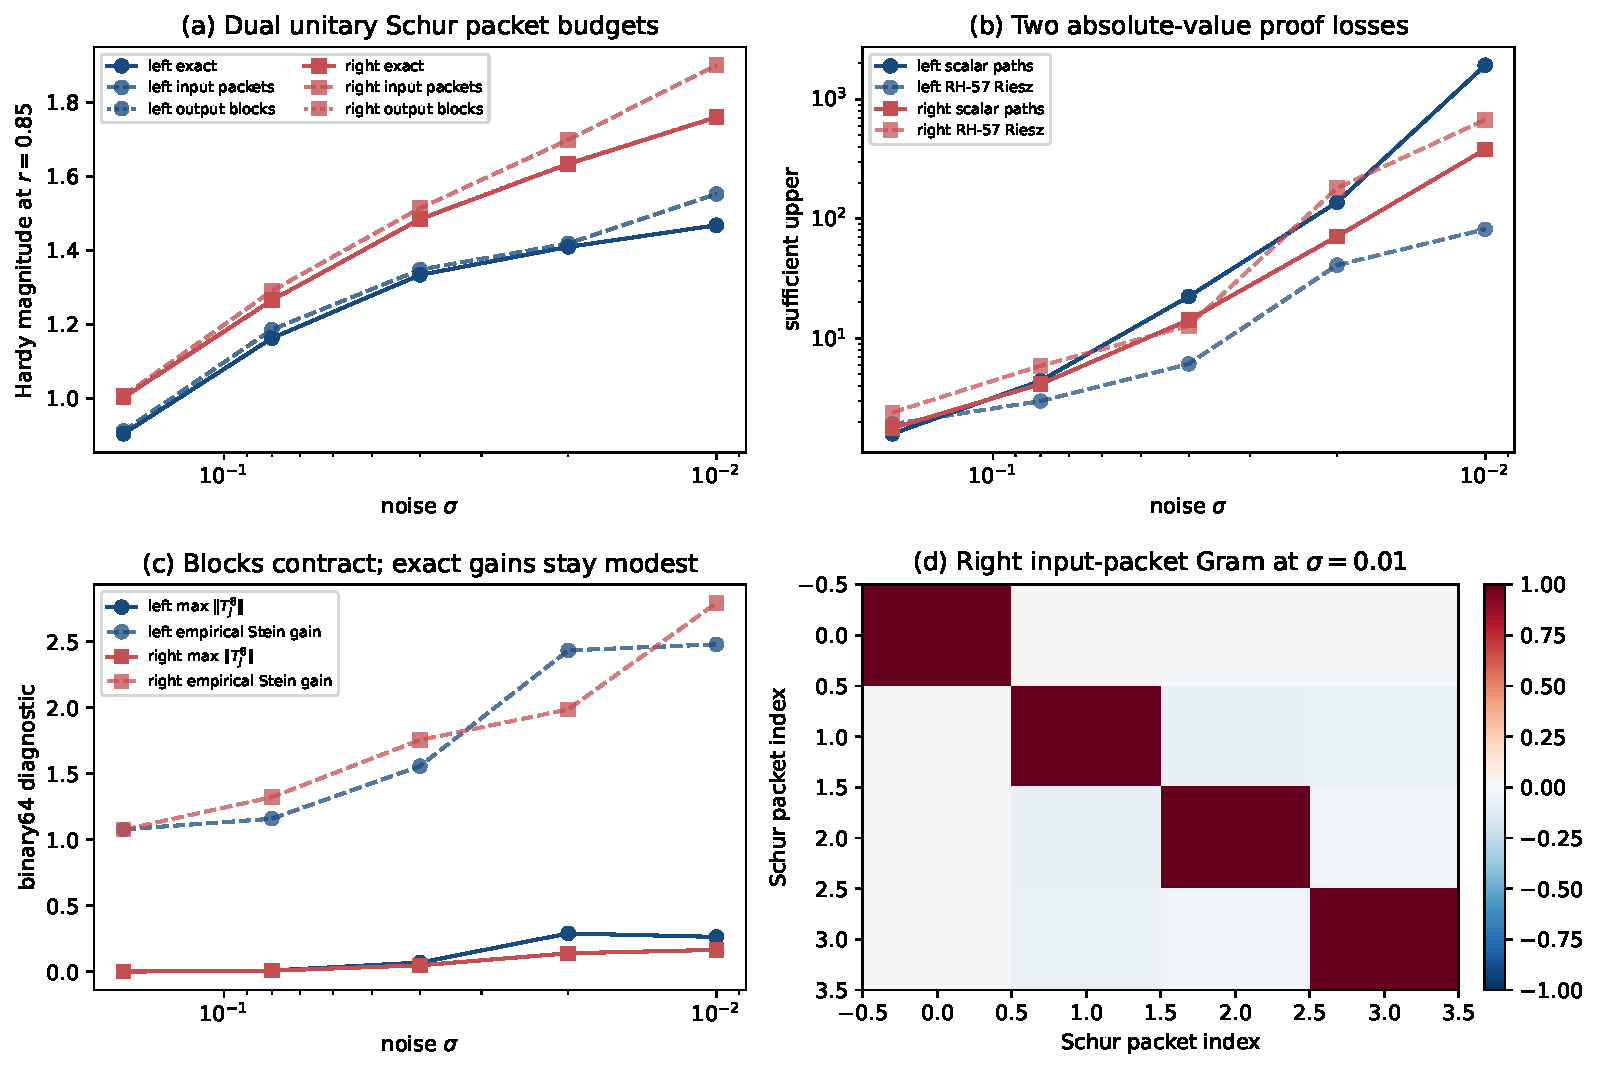
\includegraphics[width=\textwidth]{figures/time_ordered_schur_fusion.pdf}
\caption{Unitary Schur audit.  (a) Both exact packet budgets remain close to
the all-column Hardy energies.  (b) The RH-57 oblique Riesz route and the new
scalar absolute-path route lose different cancellations.  (c) All diagonal
blocks contract over eight steps while exact recursion gains stay modest.
(d) The right input-packet Gram at the smallest stored scale.}
\label{fig:audit}
\end{figure}

The maximum Schur reconstruction defect is $7.1\times10^{-15}$, the maximum
cross-Stein recursion residual is $4.7\times10^{-15}$, and the maximum
primal--dual trace discrepancy is $3.1\times10^{-15}$.  These are binary64
consistency checks, not interval enclosures.

\subsection{Outward-rounded model audit}

A 256-bit Arb calculation \citep{Johansson2017} evaluates a real
two-scalar-block upper-triangular
model.  It encloses the controllability and observability recursions, verifies
that all six Stein residual balls contain zero, checks the primal--dual and
dual packet identities, and certifies the $M=2$ scalar path upper.  No
production folded-Gaussian Schur form is interval validated.

\section{Program consequence}
\label{sec:consequence}

\begin{description}[leftmargin=4.8cm,style=nextline]
 \item[Fixed radial Riesz blocks]
 Rejected as a uniform absolute-overlap route by RH-57 obliqueness.
 \item[Unitary Schur packet coordinates]
 Quantitatively viable on the stored all-column levels.  They remove the
 projector wall and give dual positive Gram interfaces.
 \item[Scalar absolute Schur paths]
 Rejected by \cref{tab:walls}.  Block contraction alone does not prevent a
 combinatorial norm ledger from spending several powers of $\sigma$.
 \item[Remaining analytic target]
 Control the input packet Gram or output state-block Gram while preserving
 Hilbert-space square sums, phases, or an anisotropic block metric.  Do not
 replace every feed-forward path by an independent worst-case norm.
 \item[Stage A1]
 Open.  The present finite-dimensional theorem supplies a better coordinate
 system and a sharper target, not a uniform physical-family bound.
 \item[Stage A4]
 Still conditional on Stage A1; the RH-52--RH-55 interfaces remain intact.
\end{description}

The next gate is now narrower than after RH-57.  One may seek a block
observability inequality directly for $K^{\rm in}$, or construct a positive
block metric that sums Schur paths in square rather than absolutely.  The
stored data indicate that such a mechanism exists numerically, but they do
not identify a continuum-stable Schur packet basis.

\section{No arithmetic or Hilbert--Polya conclusion}

Nothing here constructs a self-adjoint operator, a $T\log T$ counting law, a
von Mangoldt or prime-power trace formula, or a zeta-zero identity.  No
Riemann-hypothesis conclusion is drawn.  The independent twin-prime branch is
not used.

\section{Reproducibility}

The archive contains the Schur algebra, tests, five-scale all-column results,
the Arb model certificate, figures, dependency hashes, and publication
artifacts.  Principal commands are
\begin{verbatim}
PYTHONDONTWRITEBYTECODE=1 /root/math/.venv/bin/pytest -q -p no:cacheprovider
PYTHONDONTWRITEBYTECODE=1 /root/math/.venv/bin/python \
  experiments/run_schur_fusion_pilot.py
PYTHONDONTWRITEBYTECODE=1 /root/math/.venv/bin/python \
  experiments/run_arb_schur_audit.py
MPLBACKEND=Agg PYTHONDONTWRITEBYTECODE=1 /root/math/.venv/bin/python \
  experiments/make_figures.py
latexmk -pdf -interaction=nonstopmode -halt-on-error main.tex
\end{verbatim}

The dual packet identities, reverse recursion, block-power gain, and scalar
path upper are analytic finite-dimensional statements.  Production Schur
forms and all fitted laws are binary64 diagnostics.  Stage A1, unconditional
intrinsic identification, and every arithmetic or Hilbert--Polya conclusion
remain outside the claims.

\bibliographystyle{plainnat}
\bibliography{references}
\end{document}
